%%%%%%%%%%%%%%%%%%%%%%%%%%%%%%%%%%%%%%%%%%%%%%%%%%%%%%%%%%%%%%%%%%%%%%%%%%%%%%%%
%%%%%%%%%%%%%%%%%%%%%%%%%%%%%%%%%%%%%%%%%%%%%%%%%%%%%%%%%%%%%%%%%%%%%%%%%%%%%%%%
%%%%%%%%%%%%%%%%%%%%%%%%%%%%%%%%%%%%%%%%%%%%%%%%%%%%%%%%%%%%%%%%%%%%%%%%%%%%%%%%
%%%%%%%%%%%%%%%%%%%%%%%%%%%%%%%%%%%%%%%%%%%%%%%%%%%%%%%%%%%%%%%%%%%%%%%%%%%%%%%%
\chapter[Performances des systèmes]
{Performances des systèmes asservis\label{chap-perf}}
%%%%%%%%%%%%%%%%%%%%%%%%%%%%%%%%%%%%%%%%%%%%%%%%%%%%%%%%%%%%%%%%%%%%%%%%%%%%%%%%
%%%%%%%%%%%%%%%%%%%%%%%%%%%%%%%%%%%%%%%%%%%%%%%%%%%%%%%%%%%%%%%%%%%%%%%%%%%%%%%%
%%%%%%%%%%%%%%%%%%%%%%%%%%%%%%%%%%%%%%%%%%%%%%%%%%%%%%%%%%%%%%%%%%%%%%%%%%%%%%%%
%%%%%%%%%%%%%%%%%%%%%%%%%%%%%%%%%%%%%%%%%%%%%%%%%%%%%%%%%%%%%%%%%%%%%%%%%%%%%%%%
\minitoc
\newpage
%%%%%%%%%%%%%%%%%%%%%%%%%%%%%%%%%%%%%%%%%%%%%%%%%%%%%%%%%%%%%%%%%%%%%%%%%%%%%%%%
%%%%%%%%%%%%%%%%%%%%%%%%%%%%%%%%%%%%%%%%%%%%%%%%%%%%%%%%%%%%%%%%%%%%%%%%%%%%%%%%
%%%%%%%%%%%%%%%%%%%%%%%%%%%%%%%%%%%%%%%%%%%%%%%%%%%%%%%%%%%%%%%%%%%%%%%%%%%%%%%%
\section{Introduction}
%%%%%%%%%%%%%%%%%%%%%%%%%%%%%%%%%%%%%%%%%%%%%%%%%%%%%%%%%%%%%%%%%%%%%%%%%%%%%%%%
%%%%%%%%%%%%%%%%%%%%%%%%%%%%%%%%%%%%%%%%%%%%%%%%%%%%%%%%%%%%%%%%%%%%%%%%%%%%%%%%
%%%%%%%%%%%%%%%%%%%%%%%%%%%%%%%%%%%%%%%%%%%%%%%%%%%%%%%%%%%%%%%%%%%%%%%%%%%%%%%%
Les performances qui vont nous interesser dans 
ce chapitre sont la \textbf{précision} et la \textbf{rapidité}.
Après avoir défini formellement ces performances en boucle ouverte, 
nous allons déterminer l'effet de l'asservissement sur chacune de 
ces performances. \textbf{Dans les deux cas, nous allons observer que 
les performances en boucle fermée dépendent directement du système 
en boucle ouverte.}
%%%%%%%%%%%%%%%%%%%%%%%%%%%%%%%%%%%%%%%%%%%%%%%%%%%%%%%%%%%%%%%%%%%%%%%%%%%%%%%%
%%%%%%%%%%%%%%%%%%%%%%%%%%%%%%%%%%%%%%%%%%%%%%%%%%%%%%%%%%%%%%%%%%%%%%%%%%%%%%%%
%%%%%%%%%%%%%%%%%%%%%%%%%%%%%%%%%%%%%%%%%%%%%%%%%%%%%%%%%%%%%%%%%%%%%%%%%%%%%%%%
\section{Précision}
%%%%%%%%%%%%%%%%%%%%%%%%%%%%%%%%%%%%%%%%%%%%%%%%%%%%%%%%%%%%%%%%%%%%%%%%%%%%%%%%
%%%%%%%%%%%%%%%%%%%%%%%%%%%%%%%%%%%%%%%%%%%%%%%%%%%%%%%%%%%%%%%%%%%%%%%%%%%%%%%%
%%%%%%%%%%%%%%%%%%%%%%%%%%%%%%%%%%%%%%%%%%%%%%%%%%%%%%%%%%%%%%%%%%%%%%%%%%%%%%%%
Un système est précis si l'écart que l'on note $\epsilon(t)$ 
entre l'entrée $e(t)$ et la sortie $s(t)$ est nul.
Dans le domaine de Laplace, cet écart devient 
\[
\epsilon(p)=E(p)-S(p).
\]
Remarquons que l'écart correspond à la grandeur élaboré par le régulateur 
(comparateur) dans un asservissement à boucle de contre réaction unitaire.

On distingue deux cas selon le régime de la réponse, en effet :
%-------------------------------------------------------------------------------
\begin{itemize}
    \item en régime permanent, cet écart $\epsilon_s$ est nommé 
		  \textbf{erreur statique; }
    \item en régime transitoire, cet écart $\epsilon(t)=e(t)-s(t)$ est 
		  nommé \textbf{erreur dynamique.}
\end{itemize}
%-------------------------------------------------------------------------------
De plus, selon le type de sollicitation on parle de :
%-------------------------------------------------------------------------------
\begin{itemize}
	\item l'\textbf{erreur indicielle} ou l'erreur de position, qui est 
		  l'erreur statique de la réponse indicielle;
	\item l'\textbf{erreur de poursuite} ou erreur de vitesse, qui est 
		  l'erreur statique de la réponse à une rampe;
	\item l'\textbf{erreur en accélération}, qui est l'erreur statique 
		  de la réponse à une parabole.
\end{itemize}
%-------------------------------------------------------------------------------
Concrétement, pour étudier l'erreur statique on cherche la limite à l'infini 
de $\epsilon(t)$ ou encore en appliquant le théorème de la valeur finale :
%-------------------------------------------------------------------------------
\begin{bequation}[ams align]
\epsilon_S=\epsilon(\infty)=\lim\limits_{t\to\infty} e(t)-s(t)
	            =\lim\limits_{p\to 0} p\big(E(p)-S(p)\big)
\end{bequation}
%-------------------------------------------------------------------------------
Rappelons que pour pouvoir appliquer ce théorème la valeur finale doit 
être finie ou en d'autre mot le système doit être stable.
%%%%%%%%%%%%%%%%%%%%%%%%%%%%%%%%%%%%%%%%%%%%%%%%%%%%%%%%%%%%%%%%%%%%%%%%%%%%%%%%
%%%%%%%%%%%%%%%%%%%%%%%%%%%%%%%%%%%%%%%%%%%%%%%%%%%%%%%%%%%%%%%%%%%%%%%%%%%%%%%%
\subsection{Précision en boucle ouverte}
%%%%%%%%%%%%%%%%%%%%%%%%%%%%%%%%%%%%%%%%%%%%%%%%%%%%%%%%%%%%%%%%%%%%%%%%%%%%%%%%
%%%%%%%%%%%%%%%%%%%%%%%%%%%%%%%%%%%%%%%%%%%%%%%%%%%%%%%%%%%%%%%%%%%%%%%%%%%%%%%%
Soit un système caractérisé par la fonction de transfert $H(p)$ 
est sollicité par l'entrée $E(p)$. La sortie $S(p)$ est alors donnée par :
%-------------------------------------------------------------------------------
\begin{center}
    \tikzsetnextfilename{sb_bloc1-chap_perf-ext}
    \input{tikz/sb_bloc1-chap_perf.tex}
\end{center}
%-------------------------------------------------------------------------------
L'erreur statique est alors donnée par :
\[
\epsilon(\infty)=\lim\limits_{p\to 0} p\big(E(p)-H(p)E(p)\big)
                =\lim\limits_{p\to 0} p\big(1-H(p)\big)E(p)
\]
%%%%%%%%%%%%%%%%%%%%%%%%%%%%%%%%%%%%%%%%%%%%%%%%%%%%%%%%%%%%%%%%%%%%%%%%%%%%%%%%
\subsubsection{Exemple d'un premier ordre}
%%%%%%%%%%%%%%%%%%%%%%%%%%%%%%%%%%%%%%%%%%%%%%%%%%%%%%%%%%%%%%%%%%%%%%%%%%%%%%%%
Prenons l'exemple d'un système du 1er ordre de fonction de transfert canonique 
$H(p)=\dfrac{K}{1+\tau p}$ que l'on sollicite avec un échelon 
d'amplitude (consigne) $E_0$.
L'erreur statique est alors donnée par :
\[
\epsilon(\infty)=\lim\limits_{p\to 0}\left(1-\dfrac{K}{1+\tau p}\right)E_0
                =(1-K)E_0
\]
Le système est prècis (c.a.d $\epsilon(\infty)=0$) si $K=1$. 
%%%%%%%%%%%%%%%%%%%%%%%%%%%%%%%%%%%%%%%%%%%%%%%%%%%%%%%%%%%%%%%%%%%%%%%%%%%%%%%%
%%%%%%%%%%%%%%%%%%%%%%%%%%%%%%%%%%%%%%%%%%%%%%%%%%%%%%%%%%%%%%%%%%%%%%%%%%%%%%%%
\subsection{Précision en boucle fermée}
%%%%%%%%%%%%%%%%%%%%%%%%%%%%%%%%%%%%%%%%%%%%%%%%%%%%%%%%%%%%%%%%%%%%%%%%%%%%%%%%
%%%%%%%%%%%%%%%%%%%%%%%%%%%%%%%%%%%%%%%%%%%%%%%%%%%%%%%%%%%%%%%%%%%%%%%%%%%%%%%%
Considérons le cas d'un système asservi de fonction de transfert $H(p)$
par une boucle de contre-réaction à retour unitaire.
%-------------------------------------------------------------------------------
\begin{center}
    \tikzsetnextfilename{sb_bloc2-chap_perf-ext}
    \begin{tikzpicture}
    \sbEntree{E}
    \sbComp{comp1}{E}
    \sbRelier[$E(p)$]{E}{comp1}
    \sbBloc[3]{H}{$H(p)$}{comp1}
    \sbRelier[$\epsilon(p)$]{comp1}{H}
    \sbSortie[3]{S}{H}
    \sbRelier[$S(p)$]{H}{S}
    \sbRenvoi[4]{H-S}{comp1}{}
\end{tikzpicture}

\end{center}
%-------------------------------------------------------------------------------
La~\gls{ftbo} est simplement donnée par $H(p)$. Dans le cas le plus
générale, il est toujours possible d'écrire une fonction de transfert
sous la forme canonique (\Cref{chap-slci}) :
\[
H_{BO}(p)=\dfrac{K}{p^\alpha}\cdot\dfrac{N(p)}{D(p)}
\]
avec $\alpha$ la classe du système en boucle ouverte, $K$ le gain statique et 
$N(p)$ et $D(p)$ deux polynômes tels que $N(0)=D(0)=1$. 
Dans le domaine de Laplace l'écart $\epsilon(p)$ s'écrit :
\[
\epsilon(p)=E(p)-S(p)=\left(1-\dfrac{H_{BO}(p)}{1+H_{BO}(p)}\right)E(p)
\]
en remplaçant $H_{BO}(p)$ par sa représentation générale:
%-------------------------------------------------------------------------------
\begin{bequation}[ams align]
    \epsilon(p)=\dfrac{p^\alpha D(p)}{p^\alpha D(p)+KN(p)}E(p)
\end{bequation}
%-------------------------------------------------------------------------------
L'erreur statique $\epsilon_s$ est alors donnée par la limite (Théorème 
de la valeur finale) :
\[
\epsilon_s=\lim\limits_{p\to 0} p\epsilon(p)=\lim\limits_{p\to 0} 
           \dfrac{p^\alpha D(p)}{p^\alpha D(p)+KN(p)}pE(p) 
\]
ou encore en utilisant les valeurs des polynômes en 0: 
%-------------------------------------------------------------------------------
\begin{bequation}[ams align]
	\epsilon_s=\lim\limits_{p\to 0} \dfrac{p^\alpha}{p^\alpha+K}pE(p)
	\label{eq-erreurStatique}
\end{bequation}
%-------------------------------------------------------------------------------
Cette erreur dépend donc de la nature de la sollicitation (c.a.d $E(p)$) et 
de la classe $\alpha$ de la fonction de transfert en boucle ouverte.

Nous allons maintenant considérer différentes types de sollicitations pour 
différentes classes de système en boucle ouverte.
%%%%%%%%%%%%%%%%%%%%%%%%%%%%%%%%%%%%%%%%%%%%%%%%%%%%%%%%%%%%%%%%%%%%%%%%%%%%%%%%
\subsubsection{Erreur statique indicielle}
%%%%%%%%%%%%%%%%%%%%%%%%%%%%%%%%%%%%%%%%%%%%%%%%%%%%%%%%%%%%%%%%%%%%%%%%%%%%%%%%
L'erreur indicielle est l'erreur entre la sortie d'un système et une 
sollicitation en échelon $e(t)=E_0u(t)$ de transformée de Laplace 
$E(p)=\dfrac{E_0}{p}$. 
Pour une telle entrée, l'erreur statique (c.f \cref{eq-erreurStatique}) 
devient :
%-------------------------------------------------------------------------------
\begin{bequation}[ams align]
\epsilon_s=\lim\limits_{p\to 0} \dfrac{p^\alpha}{p^\alpha+K}E_0
\end{bequation}
%-------------------------------------------------------------------------------
Dans le cas d'un système de classe $\alpha=0$ en boucle ouverte :
%-------------------------------------------------------------------------------
\begin{bequation}[ams align]
\epsilon_s=\lim\limits_{p\to 0} \dfrac{p^0}{p^0+K}E_0=\dfrac{E_0}{1+K}.
\end{bequation}
%-------------------------------------------------------------------------------
L'erreur est finie mais les réponses indicielles des systèmes de classe 
$\alpha=0$ en boucle ouverte ne sont pas précis.

Dans les autres cas $\alpha>0$, l'erreur statique s'annule :
%-------------------------------------------------------------------------------
\begin{bequation}[ams align]
\epsilon_s=\lim\limits_{p\to 0} \dfrac{p^\alpha}{p^\alpha+K}E_0=0
\end{bequation}
%-------------------------------------------------------------------------------
Les réponses indicielle des systèmes de classe $\alpha>0$ sont donc précis.
%%%%%%%%%%%%%%%%%%%%%%%%%%%%%%%%%%%%%%%%%%%%%%%%%%%%%%%%%%%%%%%%%%%%%%%%%%%%%%%%
\subsubsection{Erreur statique de poursuite}
%%%%%%%%%%%%%%%%%%%%%%%%%%%%%%%%%%%%%%%%%%%%%%%%%%%%%%%%%%%%%%%%%%%%%%%%%%%%%%%%
L'erreur de poursuite est l'erreur statique d'un système soumis à une rampe 
du type $e(t)=r(t)=E_0t u(t)$
de transformée de Laplace $E(p)=\dfrac{E_0}{p^2}$

Pour une telle entrée, l'erreur statique devient :
%-------------------------------------------------------------------------------
\begin{bequation}[ams align]
\epsilon_s=\lim\limits_{p\to 0} \dfrac{p^\alpha}{p^\alpha+K}\dfrac{E_0}{p}
          =\dfrac{p^{\alpha-1}}{p^\alpha+K}E_0 
\end{bequation}
%-------------------------------------------------------------------------------
Dans le cas d'un système de classe $\alpha=0$ en boucle ouverte, 
l'erreur devient :
%-------------------------------------------------------------------------------
\begin{bequation}[ams align]
\epsilon_s=\lim\limits_{p\to 0}\dfrac{p^{-1}}{p^0+K}E_0=+\infty
\end{bequation}
%-------------------------------------------------------------------------------
Le système est incapable de suivre l'entrée souhaitée.

Dans le cas d'un système de classe $\alpha=1$ en boucle ouverte, 
l'erreur devient :
%-------------------------------------------------------------------------------
\begin{bequation}[ams align]
\epsilon_s=\lim\limits_{p\to 0}\dfrac{p^0}{p+K}E_0=\dfrac{E_0}{K}
\end{bequation}
%-------------------------------------------------------------------------------
Dans le cas d'un système de classe $\alpha>1$ en boucle ouverte, 
l'erreur devient :
%-------------------------------------------------------------------------------
\begin{bequation}[ams align]
\epsilon_s=\lim\limits_{p\to 0}\dfrac{p^{\alpha-1}}{p^\alpha+K}E_0=0
\end{bequation}
%-------------------------------------------------------------------------------
Le système est donc prècis.
%%%%%%%%%%%%%%%%%%%%%%%%%%%%%%%%%%%%%%%%%%%%%%%%%%%%%%%%%%%%%%%%%%%%%%%%%%%%%%%%
\subsubsection{Erreur statique d'accélération}
%%%%%%%%%%%%%%%%%%%%%%%%%%%%%%%%%%%%%%%%%%%%%%%%%%%%%%%%%%%%%%%%%%%%%%%%%%%%%%%%
L'erreur d'accélération est l'erreur statique d'un système soumis à un signal
parabolique $e(t)=E_0t^2 u(t)$ de transformée de Laplace 
$E(p)=\dfrac{2E_0}{p^3}$

Pour une telle entrée, l'erreur statique devient :
%-------------------------------------------------------------------------------
\begin{bequation}[ams align]
\epsilon_s=\lim\limits_{p\to 0}\dfrac{p^\alpha}{p^\alpha+K}\dfrac{2E_0}{p^2}
          =\dfrac{p^{\alpha-2}}{p^\alpha+K}2E_0 
\end{bequation}
%-------------------------------------------------------------------------------
Dans le cas d'un système de classe $\alpha<2$ en boucle ouverte, 
l'erreur devient :
%-------------------------------------------------------------------------------
\begin{bequation}[ams align]
\epsilon_s=+\infty
\end{bequation}
%-------------------------------------------------------------------------------
Pour un système de classe $\alpha=2$ en boucle ouverte, 
l'erreur est finie :
%-------------------------------------------------------------------------------
\begin{bequation}[ams align]
\epsilon_s=\dfrac{2E_0}{K}
\end{bequation}
%-------------------------------------------------------------------------------
et s'annule pour $\alpha>2$
%-------------------------------------------------------------------------------
\begin{table}
    \ra{2.0}
    \centering
    \begin{tabular}{@{}P{2cm}P{2cm}P{2cm}P{2cm}P{2cm}@{}}
    \toprule
    Entrée & $\alpha=0$ & $\alpha=1$ & $\alpha=2$ & $\alpha>2$ \\
    \midrule
    $\dfrac{E_0}{p}$&$\dfrac{E_0}{1+K}$&0&0&0\\
    $\dfrac{E_0}{p^2}$&$+\infty$&$\dfrac{E_0}{K}$&0&0\\
    $\dfrac{2E_0}{p^3}$&$+\infty$&$+\infty$&$\dfrac{2E_0}{K}$&0\\
    \bottomrule
    \end{tabular}
    \caption{Résumé des erreurs statiques pour différentes 
             sollicitations et classe de système en boucle ouverte}
\end{table}
%-------------------------------------------------------------------------------
%%%%%%%%%%%%%%%%%%%%%%%%%%%%%%%%%%%%%%%%%%%%%%%%%%%%%%%%%%%%%%%%%%%%%%%%%%%%%%%%
%%%%%%%%%%%%%%%%%%%%%%%%%%%%%%%%%%%%%%%%%%%%%%%%%%%%%%%%%%%%%%%%%%%%%%%%%%%%%%%%
\subsection{Effet d'une perturbation}
%%%%%%%%%%%%%%%%%%%%%%%%%%%%%%%%%%%%%%%%%%%%%%%%%%%%%%%%%%%%%%%%%%%%%%%%%%%%%%%%
%%%%%%%%%%%%%%%%%%%%%%%%%%%%%%%%%%%%%%%%%%%%%%%%%%%%%%%%%%%%%%%%%%%%%%%%%%%%%%%%
%%%%%%%%%%%%%%%%%%%%%%%%%%%%%%%%%%%%%%%%%%%%%%%%%%%%%%%%%%%%%%%%%%%%%%%%%%%%%%%%
\subsubsection{Cas générale}
%%%%%%%%%%%%%%%%%%%%%%%%%%%%%%%%%%%%%%%%%%%%%%%%%%%%%%%%%%%%%%%%%%%%%%%%%%%%%%%%
On considère maintenant l'effet d'une perturbation sur la précision d'un 
système asservis.
Sans perte de généralité, on ne considèrera que le cas d'une perturbation 
en entrée (c'est à dire en amont d'un système linéaire défini par une fonction 
de transfert $H_2(p)$), la présence d'un correcteur $H_1(p)$ n'est pas 
obligatoire mais facilite l'interprétation des résultats.

Considérons le schéma bloc suivant avec les fonctions de transfert $H_1(p)$ 
et $H_2(p)$ de forme canonique :
%-------------------------------------------------------------------------------
\begin{align*}
    H_1(p)=\dfrac{K_1}{p^{\alpha_1}}\dfrac{N_1(p)}{D_1(p)} \\
    H_2(p)=\dfrac{K_2}{p^{\alpha_2}}\dfrac{N_2(p)}{D_2(p)}
\end{align*}
%-------------------------------------------------------------------------------
de les gains statiques $K_i$, de classe $\alpha_i$, de polynômes $N_i(p)$
et $D_i(p)$ tels que $N_i(0)=1$ et $D_i(0)=1$.
%-------------------------------------------------------------------------------
\begin{center}
    \tikzsetnextfilename{reduc_mult1-chap_perf-ext}
    \begin{tikzpicture}
    \cpbruni[$E(p)$][$\epsilon(p)$][$H_1(p)$][][ ][$P(p)$][$H_2(p)$][][$S(p)$]
\end{tikzpicture}

\end{center}
%-------------------------------------------------------------------------------
Pour déterminer l'écart, il nous faut déterminer la sortie globale $S(p)$ pour
des entrées multiples (c.f~\Cref{chap-schemabloc}-\cref{sec-multE}).
Cette sortie est sous la forme :
\[
S(p)=H_{P=0}E(p)+H_{E=0}P(p)
\]
c'est à dire que c'est la somme des contributions des deux entrées prises
séparément.
L'écart est alors donné par 
\[
\epsilon(p)=E(p)-S(p)=\left(1-H_{P=0}\right)E(p)-H_{E=0}P(p)
\]
ou encore en notant $\epsilon_S(p)=\left(1-H_{P=0}\right)E(p)$ et 
$\epsilon_P(p)=-H_{E=0}P(p)$
\[
    \epsilon(p)=\epsilon_S(p) + \epsilon_P(p)
\]
Le premier terme correspond à l'écart de l'asservissement que nous avons 
déjà étudié précedemment, le second terme, que l'on 
note $\epsilon_P(p)$, est la contribution à l'écart dû à la perturbation.
La fonction de transfert de l'asservissement est donnée par :
\[
H_{P=0}=\dfrac{H_1H_2(p)}{1+H_1(p)H_2(p)} 
\]
Dans le cas de la régulation d'un système asservis, il est nécessaire de 
rejeter cette contribution.

La fonction de transfert $H_{E=0}$, de la régulation, correspondant à une 
consigne nulle, s'obtient en considérant le schéma-bloc suivant :
%-------------------------------------------------------------------------------
\begin{center}                                                  
    \tikzsetnextfilename{pert1-chap_perf-ext}
    \begin{tikzpicture}                                         
    \bbr[$P(p)$][][$H_2(p)$][][$S(p)$][$H_1(p)$][][ ] 
\end{tikzpicture}                                           

\end{center}                                                    
%-------------------------------------------------------------------------------
\newcommand{\pau}{p^{\alpha_1}}
\newcommand{\pad}{p^{\alpha_2}}
en boucle fermée, on a alors:
\[
H_{E=0}(p)=\dfrac{H_2(p)}{1+H_1(p)H_2(p)}
\]
en remplaçant par leurs formes canoniques générales :
\[
H_{E=0}(p)=
\dfrac{\pau K_2N_2(p)D_1(p)}{\pau\pad D_1(p)D_2(p)+K_1K_2N_1(p)N_2(p)}
\]
Examinons l'erreur en régime permanent pour une perturbation constante.
C'est à dire pour perturbation $P(p)$ en échelon telle que 
$P(p)=\dfrac{P_0}{p}$. L'erreur dû à la perturbation en régime permanent 
est alors :
%-------------------------------------------------------------------------------
\begin{align*}
    \epsilon_P&=\lim\limits_{p\to0} p\epsilon_P(p)\\
    \epsilon_P&=\lim\limits_{p\to0} -H_{E=0}P_0\\
    \epsilon_P&=\lim\limits_{p\to0}\dfrac{\pau K_2}{\pau\pad+K_1K_2}P_0
\end{align*}
%-------------------------------------------------------------------------------
\textbf{La perturbation est rejétée ($\epsilon_P=0$) si $\alpha_1>0$, 
c'est à dire s'il existe au moins un intégrateur en amont de la perturbation.}
En effet si $\alpha_1=0$, l'erreur dû à la perturbation est finie et 
donnée par :
\[
    \begin{cases}
        \alpha_2=0 & \epsilon_P=\dfrac{K_2}{1+K_1K_2}P_0 \\[1.5em]
        \alpha_2>0 & \epsilon_P=\dfrac{P_0}{K_1}
    \end{cases}
\]
\newpage
%%%%%%%%%%%%%%%%%%%%%%%%%%%%%%%%%%%%%%%%%%%%%%%%%%%%%%%%%%%%%%%%%%%%%%%%%%%%%%%%
\subsubsection{Exemple de rejet de perturbation}
%%%%%%%%%%%%%%%%%%%%%%%%%%%%%%%%%%%%%%%%%%%%%%%%%%%%%%%%%%%%%%%%%%%%%%%%%%%%%%%%
Nous allons voir ici le rejet d'une perturbation d'un système du premier ordre. 
On considère le système du premier ordre, en boucle ouverte, placé dans une 
boucle de contre réaction unitaire avec un intégrateur comme ci-dessous :
%-------------------------------------------------------------------------------
\begin{center}                           
    \tikzsetnextfilename{pert2-chap_perf-ext}
    %%%%%%%%%%%%%%%%%%%%%%%%%%%%%%%%%%%%%%%%%%%%%%%%%%%%%%%%%%%%%%%%%%%%%%%%%%%%%%%%
%   Nom des noeuds
%                        P1            P2 
%                        |             |
%                        |             | 
%   E ---- a ---- b ---- c ---- d ---- e ---- S
%          |                                  |
%          |                                  |
%           ------------ g ---- f ------------ 
%                        |
%                        |
%                        P3
% E  : entrée
% a  : comparateur/régulateur
% b  : correcteur 
% c  : sommateur1 (perturbation)
% d  : système 
% e  : sommateur2 (perturbation)
% f  : capteur
% g  : sommateur3 (perturbation/bruit)
% P1 : noeud décalé pour la perturbation
% P2 : noeud décalé pour la perturbation
% P3 : noeud décalé pour la perturbation
% S  : sortie
% r  : noeud décalé pour le retour
%%%%%%%%%%%%%%%%%%%%%%%%%%%%%%%%%%%%%%%%%%%%%%%%%%%%%%%%%%%%%%%%%%%%%%%%%%%%%%%%
\begin{tikzpicture}                  
    \sbEntree{E}
    \sbComp{comp1}{E}
    \sbRelier[$E(p)$]{E}{comp1}
    \sbBloc[3]{C}{$\dfrac{1}{p}$}{comp1}
    \sbRelier[$\epsilon(p)$]{comp1}{C}
    \sbBloc[3]{H}{$\dfrac{1}{p+1}$}{C}
    \sbRelier[]{C}{H}
    \sbSortie[3]{S}{H}
    \sbRelier[$S(p)$]{H}{S}
    \sbRenvoi[4]{H-S}{comp1}{}
\end{tikzpicture}                    

\end{center}                             
%-------------------------------------------------------------------------------
On souhaite réguler ce système pour une consigne en échelon.
D'après les résultats précédents, l'erreur statique de position est nulle 
en asservissement puisque le système présente au moins un intégrateur. 
Pour observer le rejet de la perturbation, nous allons considérer 
deux positions possibles pour la perturbation (avant et après 
l'intégrateur). On considère une perturbation constante telle 
que $P(p)=e^{-\tau p}\dfrac{P_0}{p}$ retardée d'un temps $\tau>0$. 
%%%%%%%%%%%%%%%%%%%%%%%%%%%%%%%%%%%%%%%%%%%%%%%%%%%%%%%%%%%%%%%%%%%%%%%%%%%%%%%%
\paragraph{Si l'intégrateur est en aval de la perturbation}
%%%%%%%%%%%%%%%%%%%%%%%%%%%%%%%%%%%%%%%%%%%%%%%%%%%%%%%%%%%%%%%%%%%%%%%%%%%%%%%%
Dans un tel cas l'erreur dû à la perturbation est donnée par :
\[
\epsilon_P=\lim\limits_{p\to0}p\epsilon_P(p)=
\lim\limits_{p\to0}\dfrac{e^{-\tau p}}{p(p+1)+1}P_0=P_0
\]
L'erreur statique de position totale est donc non nulle. La perturbation
n'est pas rejétée comme on peut le voir sur la simulation de la réponse
temporelle globale de ce système (c.f~\cref{fig-pert1}).
%-------------------------------------------------------------------------------
\begin{figure}[!h]
    \centering
    \tikzsetnextfilename{pert1_data-chap_perf-ext}
    \begin{tikzpicture}
    \begin{axis}
    [   legend style={draw=none,font=\normalsize},
        legend pos=outer north east,
        axis line style = thick,
        width=0.45\textwidth,
        xmin=0,
        xmax=30,
        ymin=0,
        ymax=1.75,
        xlabel={$t$},
        ylabel={$s(t)$},
        label style={font=\Large},
        legend cell align={left},
    ]%
        \addplot[mark=none,vtb] table {pert1_data.tab};
        \addplot[col4,thick,domain=0:15] {1};   %échelon
        \addplot[col4,thick,domain=15:30] {1.5}; %pertubation
        \addplot[col4,thick,domain=-2:0] {0};
        \draw[col4,thick,dashed] (0,0)--(0,1);   %échelon
        \draw[col4,thick,dashed] (15,1)--(15,1.5);   %échelon
    \end{axis}
    \begin{scope}[shift={(-10,2.3)}]
        \sbEntree{E}
        \sbCompSum{comp1}{E}{+}{-}{+}{}
        \sbRelier[$E(p)$]{E}{comp1}
        \sbBloc[2.5]{C}{$\dfrac{1}{p}$}{comp1}
        \sbRelier[$\epsilon(p)$]{comp1}{C}
        \sbBloc[3]{H}{$\dfrac{1}{p+1}$}{C}
        \sbRelier[]{C}{H}
        \sbSortie[3]{S}{H}
        \sbRelier[$S(p)$]{H}{S}
        \sbRenvoi[4]{H-S}{comp1}{}
        \sbDecaleNoeudy[-2.5]{comp1}{P}
        \sbRenvoiF[-2.5]{P}{comp1}{$P(p)$}
    \end{scope}
\end{tikzpicture}

    \caption{Effet de la perturbation sur la réponse temporelle dans le cas
             où l'intégrateur est en aval de la perturbation. La simulation 
             de la réponse temporelle est obtenue pour les paramètres suivants:
             $E_0=1$, $P_0=0.5$ et $\tau=15$\label{fig-pert1}}
\end{figure}
%-------------------------------------------------------------------------------
%%%%%%%%%%%%%%%%%%%%%%%%%%%%%%%%%%%%%%%%%%%%%%%%%%%%%%%%%%%%%%%%%%%%%%%%%%%%%%%%
\paragraph{Si l'intégrateur est en amont de la perturbation}
%%%%%%%%%%%%%%%%%%%%%%%%%%%%%%%%%%%%%%%%%%%%%%%%%%%%%%%%%%%%%%%%%%%%%%%%%%%%%%%%
Dans un tel cas l'erreur dû à la perturbation est donnée par :
\[
\epsilon_P=\lim\limits_{p\to0}\dfrac{pe^{-\tau p}}{p(p+1)+1}P_0=0
\]
L'erreur statique de position totale est donc nulle. La perturbation
est rejétée, comme on peut le voir sur la simulation de la réponse
temporelle globale de ce système (c.f~\cref{fig-pert2}).
%-------------------------------------------------------------------------------
\begin{figure}[!h]
    \centering
    \tikzsetnextfilename{pert2_data-chap_perf-ext}
    \begin{tikzpicture}
    \begin{axis}
    [   legend style={draw=none,font=\normalsize},
        legend pos=outer north east,
        axis line style = thick,
        width=0.45\textwidth,
        xmin=0,
        xmax=30,
        ymin=0,
        ymax=1.75,
        xlabel={$t$},
        ylabel={$s(t)$},
        label style={font=\Large},
        legend cell align={left},
    ]%
        \addplot[mark=none,vtb] table {pert2_data.tab};
        \addplot[col4,thick,domain=0:15] {1};   %échelon
        \addplot[col4,thick,domain=15:30] {1.5}; %pertubation
        \addplot[col4,thick,domain=-2:0] {0};
        \draw[col4,thick,dashed] (0,0)--(0,1);   %échelon
        \draw[col4,thick,dashed] (15,1)--(15,1.5);   %échelon
    \end{axis}
    \begin{scope}[shift={(-10,2.3)}]
        \sbEntree{E1}
        \sbComp{comp}{E1}
        \sbRelier[$E(p)$]{E1}{comp}
        \sbBloc[2]{C1}{$\dfrac{1}{p}$}{comp}
        \sbRelier[$\epsilon(p)$]{comp}{C1}
        \sbCompSum[4.0]{pert}{C1}{+}{}{+}{}
        \sbRelier[]{C1}{pert}
        \sbBloc[1.5]{B1}{$\dfrac{1}{p+1}$}{pert}
        \sbRelier{pert}{B1}
        \sbSortie[2.5]{S1}{B1}
        \sbRelier[$S(p)$]{B1}{S1}
        \sbRenvoi[4]{B1-S1}{comp}{}
        \sbDecaleNoeudy[-2.5]{pert}{P}
        \sbRenvoiF[-2.5]{P}{pert}{$P(p)$}
    \end{scope}
\end{tikzpicture}

    \caption{Effet de la perturbation sur la réponse temporelle dans le cas
             où l'intégrateur est en amont de la perturbation. La simulation
             de la réponse temporelle est obtenue pour les paramètres suivants: 
             $E_0=1$, $P_0=0.5$ et $\tau=15$\label{fig-pert2}}
\end{figure}
%-------------------------------------------------------------------------------
\clearpage
%%%%%%%%%%%%%%%%%%%%%%%%%%%%%%%%%%%%%%%%%%%%%%%%%%%%%%%%%%%%%%%%%%%%%%%%%%%%%%%%
%%%%%%%%%%%%%%%%%%%%%%%%%%%%%%%%%%%%%%%%%%%%%%%%%%%%%%%%%%%%%%%%%%%%%%%%%%%%%%%%
%%%%%%%%%%%%%%%%%%%%%%%%%%%%%%%%%%%%%%%%%%%%%%%%%%%%%%%%%%%%%%%%%%%%%%%%%%%%%%%%
\section{Rapidité\label{sec-rapidite}}
%%%%%%%%%%%%%%%%%%%%%%%%%%%%%%%%%%%%%%%%%%%%%%%%%%%%%%%%%%%%%%%%%%%%%%%%%%%%%%%%
%%%%%%%%%%%%%%%%%%%%%%%%%%%%%%%%%%%%%%%%%%%%%%%%%%%%%%%%%%%%%%%%%%%%%%%%%%%%%%%%
%%%%%%%%%%%%%%%%%%%%%%%%%%%%%%%%%%%%%%%%%%%%%%%%%%%%%%%%%%%%%%%%%%%%%%%%%%%%%%%%
La rapidité est un critère important dans le contexte du contrôle des 
systèmes dynamiques. Cette rapidité correspond à la durée que met un 
système pour atteindre le régime permanent. Ce critère de performance 
dépend donc directement du transitoire de la réponse temporelle. 
En générale, la valeur finale de la réponse d'un système est atteinte de 
façon asymptotique. C'est pourquoi, ce critère est généralement évalué 
relativement à la valeur finale de la réponse indicielle. 
Dans le cas des systèmes en boucle ouverte, nous ne rappelerons que les 
résultats obtenues dans les chapitres précédents. 
L'objectif principale est ici d'évaluer l'effet du bouclage sur ce critère 
de performance.
%%%%%%%%%%%%%%%%%%%%%%%%%%%%%%%%%%%%%%%%%%%%%%%%%%%%%%%%%%%%%%%%%%%%%%%%%%%%%%%%
%%%%%%%%%%%%%%%%%%%%%%%%%%%%%%%%%%%%%%%%%%%%%%%%%%%%%%%%%%%%%%%%%%%%%%%%%%%%%%%%
\subsection{Réponse temporelle}
%%%%%%%%%%%%%%%%%%%%%%%%%%%%%%%%%%%%%%%%%%%%%%%%%%%%%%%%%%%%%%%%%%%%%%%%%%%%%%%%
%%%%%%%%%%%%%%%%%%%%%%%%%%%%%%%%%%%%%%%%%%%%%%%%%%%%%%%%%%%%%%%%%%%%%%%%%%%%%%%%
Dans la pratique, on caractérise la rapidité d'une réponse temporelle par 
l'intermédiaire de deux valeurs : $t_{5\%}$ le \textbf{temps de réponse à 5\%}
et $t_m$ le \textbf{temps de montée}. 
On rappel ici les définitions de ces deux temps ainsi que 
les résultats obtenues au~\cref{chap-model} pour les systèmes modèles.
%%%%%%%%%%%%%%%%%%%%%%%%%%%%%%%%%%%%%%%%%%%%%%%%%%%%%%%%%%%%%%%%%%%%%%%%%%%%%%%%
\subsubsection{Temps de réponse à 5\% et temps de montée}
%%%%%%%%%%%%%%%%%%%%%%%%%%%%%%%%%%%%%%%%%%%%%%%%%%%%%%%%%%%%%%%%%%%%%%%%%%%%%%%%
Le temps de réponse à 5\% d'un système correspond au temps mis par la réponse 
pour atteindre 5\% de sa valeur finale $s(\infty)$. Dans le cas où la réponse 
tend asymptotiquement en oscillant vers la valeur finale, le temps de
réponse à 5\% correspond au temps pour lequel le signal de la réponse reste
dans une bande à 5\% autour de la valeur finale. 
%-------------------------------------------------------------------------------
\begin{figure}[!h]
    \centering
    \tikzsetnextfilename{rapidite_t5pc_1-chap_perf-ext}
    \begin{tikzpicture}
    \pgfmathsetmacro{\kK}{1.75}
    \pgfmathsetmacro{\tT}{1.0}
    \pgfmathsetmacro{\mC}{1.6625}
    \pgfmathsetmacro{\pC}{1.8375}
    \begin{axis}
    [   axis line style = thick,
	ticks=none,
        width=0.45\textwidth,
        axis x line=center,
        axis y line=center,
        xmin=-1,
        xmax=6,
        ymin=0,
        ymax=2.25,
        xlabel={$t$},
        ylabel={$s(t)$},
        xlabel style={below right},
        ylabel style={above left},
        clip=false
    ]
    \addplot[signalb,domain=-1:0] {0};
    \addplot[signalb,domain=0:6]  {\kK*(1-exp(-x/\tT))};
    \draw[dtb] (axis cs:0,\mC) -- (axis cs:6,\mC);
    \draw[dtb] (axis cs:0,\pC) -- (axis cs:6,\pC);
    \draw[dvtr] (axis cs:3*\tT,0) node[below] {\small $t_{5\%}$} 
             -- (axis cs:3*\tT,\mC);
    \node[right] at (axis cs:6,\kK) {\small $s(\infty)$};
    \draw[dtb,{Latex[length=1.25mm]}-{Latex[length=1.25mm]}](axis cs:-0.25,\mC) 
    -- node[midway,left] {\small $\pm5\%$} (axis cs:-0.25,\pC);
    \draw[fill=col4,col4] (axis cs:3*\tT,\mC) circle[radius=1.5pt] ;
    \end{axis}
\end{tikzpicture}

    \tikzsetnextfilename{rapidite_t5pc_2-chap_perf-ext}
    \pgfmathdeclarefunction{func}{1}{%
    \pgfmathparse{%
    1-((1./sqrt(1-#1*#1))*exp(-#1*x)*
    sin(deg(x)*sqrt(1-#1*#1)+atan(sqrt(1-#1*#1)/#1)))
    }%
}
\begin{tikzpicture}
    \pgfmathsetmacro{\kk}{1.75}
    \pgfmathsetmacro{\xm}{10.0}
    \pgfmathsetmacro{\ym}{1.5*\kk}
    \pgfmathsetmacro{\mc}{0.95*\kk}
    \pgfmathsetmacro{\pc}{1.05*\kk}
    \pgfmathsetmacro{\a}{0.48}               % amortissement xi
    \pgfmathsetmacro{\tr}{5.2}               % temps de réponse à 5%
    \begin{axis}
    [   axis line style = thick,
        axis x line=center,
        axis y line=center,
	ticks=none,
        width=0.45\textwidth,
        xmin=-1.0,
        xmax=\xm,
        ymin=0,
        ymax=2.25,
        xlabel={$t$},
        ylabel={$s(t)$},
        xlabel style={below right},
        ylabel style={above left},
        clip=false,
    ]
    \addplot[signalb,domain=-1:0] {0}                ;
    \addplot[signalb,domain=0:\xm] {\kk*func(\a)}    ;
    \draw[dtb] (axis cs:0,\mc) -- (axis cs:\xm,\mc)  ;
    \draw[dtb] (axis cs:0,\pc) -- (axis cs:\xm,\pc)  ;
    \node[right] at (axis cs:\xm,\kk) {\small $s(\infty)$}  ;
    \draw[dvtr] (axis cs:\tr,0) node[below] {\small $t_{5\%}$} 
             -- (axis cs:\tr,\pc);
    \draw[dtb,{Latex[length=1.25mm]}-{Latex[length=1.25mm]}](axis cs:-0.25,\mc) 
    -- node[midway,left] {\small $\pm5\%$} (axis cs:-0.25,\pc);
    \draw[fill=col4,col4] (axis cs:\tr,\pc) circle (1.5pt);
    \end{axis}
\end{tikzpicture}

    \caption{Définition du temps de réponse à 5\% : (à gauche) dans le cas
             d'une résonse temporelle sans pseudo-oscillations et (à droite) 
             dans le cas d'un réponse temporelle avec pseudo-oscillations}
\end{figure}
%-------------------------------------------------------------------------------
Il apparait clair que dans le cas d'une réponse présentant des oscillations,
le temps de réponse à 5\% va dépendre de l'amplitude et la période des 
pseudo-oscillations. Dans le cas où l'on souhaite caractériser la rapidité
indépendamment de ces oscillations, on utilisera le temps de montée.

Le temps de montée $t_m$ est le temps mis par la réponse temporelle d'un 
système pour passer de 10\% à 90\% de la valeur finale. Il existe une autre 
définition du temps de montée. Pour celle-ci le temps de montée (que nous 
noterons $t_{M}$ ) correspond à la durée au bout de laquelle la 
réponse passe pour la première fois par la valeur finale. Cependant, 
il faut remarquer que pour les réponses monotones la valeur finale n'est 
jamais atteinte en un temps fini. Cette dernière définition
n'a donc de sens qu'en régime pseudo-périodique.
Quelque soit la grandeur utilisée pour caractériser les performances de rapidité
d'un système linéaire, on pourra simplement dire que 
\textbf{plus le temps de réponse à 5\% et le temps de montée $t_m$ seront 
faibles plus le système sera rapide.}
%-------------------------------------------------------------------------------
\begin{figure}[!h]
    \centering
    \tikzsetnextfilename{rapidite_tm_1-chap_perf-ext}
    \begin{tikzpicture}
    \pgfmathsetmacro{\kk}{1.75}
    \pgfmathsetmacro{\t}{1.5}
    \pgfmathsetmacro{\mc}{0.10*\kk}
    \pgfmathsetmacro{\pc}{0.90*\kk}
    \pgfmathsetmacro{\xm}{10}
    \pgfmathsetmacro{\tu}{0.15}  % tm = td-tu
    \pgfmathsetmacro{\td}{3.5} 
    \begin{axis}
    [   axis line style = thick,
	ticks=none,
        width=0.45\textwidth,
        axis x line=center,
        axis y line=center,
        xmin=-1,
        xmax=\xm,
        ymin=0,
        ymax=2.25,
        xlabel={$t$},
        ylabel={$s(t)$},
        xlabel style={below right},
        ylabel style={above left},
        clip=false,
    ]
    \addplot[signalb,domain=-1:0] {0};
    \addplot[signalb,domain=0:\xm]  {\kk*(1-exp(-x/\t))};
    \draw[dtb] (axis cs:0,\mc) node[left] {\small 10\%}-- (axis cs:\xm,\mc);
    \draw[dtb] (axis cs:0,\pc) node[left] {\small 90\%}-- (axis cs:\xm,\pc);
    \draw[dvtr] (axis cs:\tu,0) node[below] {\small $t_1$} -- (axis cs:\tu,\mc);
    \draw[dvtr] (axis cs:\td,0) node[below] {\small $t_2$} -- (axis cs:\td,\pc);
    \node[right] at (axis cs:\xm,\kk) {\small $s(\infty)$};
    \draw[fill=col4,col4] (axis cs:\tu,\mc) circle[radius=1.25pt];
    \draw[fill=col4,col4] (axis cs:\td,\pc) circle[radius=1.25pt];
    \draw[vtr,{Latex[length=2mm]}-{Latex[length=2mm]}](axis cs:\tu,-0.4)
    -- node[midway,below] {\small $t_m=t_2-t_1$} (axis cs:\td,-0.4);
    \end{axis}
\end{tikzpicture}

    \tikzsetnextfilename{rapidite_tm_2-chap_perf-ext}
    \pgfmathdeclarefunction{func}{1}{%
    \pgfmathparse{%
    1-((1./sqrt(1-#1*#1))*exp(-#1*x)*
    sin(deg(x)*sqrt(1-#1*#1)+atan(sqrt(1-#1*#1)/#1)))
    }%
}
\begin{tikzpicture}
    \pgfmathsetmacro{\kk}{1.75}
    \pgfmathsetmacro{\xm}{8.0}
    \pgfmathsetmacro{\ym}{1.5*\kk}
    \pgfmathsetmacro{\mc}{0.10*\kk}
    \pgfmathsetmacro{\pc}{0.90*\kk}
    \pgfmathsetmacro{\a}{0.55}               % amortissement xi
    \pgfmathsetmacro{\tu}{0.51}  % tm = td-tu
    \pgfmathsetmacro{\td}{2.2} 
    \pgfmathsetmacro{\tvf}{2.6} % tm,vf
    \begin{axis}
    [   axis line style = thick,
        axis x line=center,
        axis y line=center,
	ticks=none,
        width=0.45\textwidth,
        xmin=-1.0,
        xmax=\xm,
        ymin=0,
        ymax=2.25,
        xlabel={$t$},
        ylabel={$s(t)$},
        xlabel style={below right},
        ylabel style={above left},
        clip=false,
    ]
    \addplot[signalb,domain=-1:0] {0}                ;
    \addplot [signalb,domain=0:\xm] {\kk*func(\a)}   ;
    \draw[dtb] (axis cs:0,\mc) node[left] {\small 10\%}-- (axis cs:\xm,\mc);%10%
    \draw[dtb] (axis cs:0,\pc) node[left] {\small 90\%}-- (axis cs:\xm,\pc);%90%
    \draw[dtn] (axis cs:0,\kk) -- (axis cs:\xm,\kk);                  % vf
    \node[right] at (axis cs:\xm,\kk) {\small $s(\infty)$}  ;
    \draw[fill=col4,col4] (axis cs:\tu,\mc) circle (1.25pt);
    \draw[fill=col4,col4] (axis cs:\td,\pc) circle (1.25pt);
    \draw[fill=black]   (axis cs:\tvf,\kk) circle (1.25pt);
    \draw[dvtr] (axis cs:\tu,0) node[below] {\small$t_1$} -- (axis cs:\tu,\mc);
    \draw[dvtr] (axis cs:\td,0) node[below,xshift=-0.5em] {\small$t_2$} 
        -- (axis cs:\td,\pc);
    \draw[dvtn] (axis cs:\tvf,0)node[below,xshift=0.75em]  {\small$t_{M}$} 
        -- (axis cs:\tvf,\kk);
    \draw[vtr,{Latex[length=2mm]}-{Latex[length=2mm]}](axis cs:\tu,-0.4)
    -- node[midway,below] {$t_m=t_2-t_1$} (axis cs:\td,-0.4);
    \end{axis}
\end{tikzpicture}

    \caption{Définition du temps de montée : (à gauche) dans le cas
             d'une résonse temporelle sans pseudo-oscillations et (à droite) 
             dans le cas d'un réponse temporelle avec pseudo-oscillations}
\end{figure}
%-------------------------------------------------------------------------------
%\clearpage
%%%%%%%%%%%%%%%%%%%%%%%%%%%%%%%%%%%%%%%%%%%%%%%%%%%%%%%%%%%%%%%%%%%%%%%%%%%%%%%%
\subsubsection{Système du premier ordre}
%%%%%%%%%%%%%%%%%%%%%%%%%%%%%%%%%%%%%%%%%%%%%%%%%%%%%%%%%%%%%%%%%%%%%%%%%%%%%%%%
La réponse indicielle $s(t)$, à un échelon unitaire, 
d'un système du premier ordre est donnée par l'\cref{eq-1er_ind} 
du~\cref{chap-model}, à savoir :
\[
s(t)=K\left(1-e^{-t/\tau}\right)
\]
Le temps de réponse à 5\%, $t_{5\%}$, est tel que $s(t_{5\%})=0.95K$, 
\[
t_{5\%}=-\tau\log{0.05}\sim3\tau.
\]
Le temps de montée $t_m=t_2-t_1$ avec $t_1$ et $t_2$, les temps tels que :
%-------------------------------------------------------------------------------
\begin{align*}
    s(t_1)&=0.1K\\
    s(t_2)&=0.9K\\
    t_m   &=-\tau\log{\dfrac{0.1}{0.9}}\sim2.2\tau
\end{align*}
%-------------------------------------------------------------------------------
Le temps de réponse à 5\% et le temps de montée $t_m$ dépendent 
directement de la constante. Ce qui permet de vérifier que 
\textbf{plus la constante de temps $\tau$ d'un système du premier
ordre est faible plus le système est rapide.}
%%%%%%%%%%%%%%%%%%%%%%%%%%%%%%%%%%%%%%%%%%%%%%%%%%%%%%%%%%%%%%%%%%%%%%%%%%%%%%%%
\paragraph{Effet du bouclage sur un système du premier ordre}
%%%%%%%%%%%%%%%%%%%%%%%%%%%%%%%%%%%%%%%%%%%%%%%%%%%%%%%%%%%%%%%%%%%%%%%%%%%%%%%%
Nous avons montré au~\cref{chap-asservis} que les paramètres de 
la~\gls{ftbf} d'un système du premier ordre $(K_{BF},\tau_{BF})$ peuvent 
être obtenues à partir des paramètres de la~\gls{ftbo}. Notamment les relations
suivantes :
%-------------------------------------------------------------------------------
\begin{align*}
       K_{BF}&=\dfrac{K}{1+K}\\
    \tau_{BF}&=\dfrac{\tau}{1+K}
\end{align*}
%-------------------------------------------------------------------------------
Il est alors possible de modifier la constante de temps en boucle fermée en 
modifiant la valeur du gain statique en boucle ouverte. \textbf{Pour augmenter
la rapidité d'un système, on augmentera le gain statique de la~\gls{ftbo} pour
diminuer les temps de réponse et de montée.}
%%%%%%%%%%%%%%%%%%%%%%%%%%%%%%%%%%%%%%%%%%%%%%%%%%%%%%%%%%%%%%%%%%%%%%%%%%%%%%%%
\subsubsection{Système du second ordre}
%%%%%%%%%%%%%%%%%%%%%%%%%%%%%%%%%%%%%%%%%%%%%%%%%%%%%%%%%%%%%%%%%%%%%%%%%%%%%%%%
Comme nous l'avons dejà souligné au~\cref{chap-model}, dans le cas d'un système
du second ordre, il n'existe pas de forme analytique simple pour déterminer 
le temps de réponse à 5\%. Nous savons cependant que ce temps de réponse est 
une fonction du coefficient d'amortissement $\xi$ et qu'il dépend également 
de la pulsation propre du système $\omega_0$.

En générale, pour déterminer le temps de réponse à 5\%, on utilise l'abaque de 
la~\cref{fig-2nd_temps_reponse_1}. Sur cette figure nous avons représenté
le temps de réponse à 5\% et le temps de montée réduits par rapport à la
pulsation propre $\omega_0$. On observe en effet que \textbf{pour un même 
coefficient d'amortissement, plus la pulsation propre augmente plus 
le temps de réponse diminue, donc plus le système est rapide.}

Nous pouvons relever sur ces abaques les coefficients d'amortissement donnant
lieu au système le plus rapide selon le régime du second ordre accepté.
\textbf{Dans le cas où les dépassements ne sont pas autorisés (c.a.d régime 
apériodique ($\xi>1$)), le système est le plus rapide pour 
$t_{5\%}\cdot\omega_0\sim5$. Dans le cas où un dépassement relatif est 
autorisé, le temps de réponse minimal est obtenu pour $\xi\sim 0.7$ soit
pour $t_{5\%}\cdot\omega_0\sim3$.}

Pour des valeurs de $\xi<1$, il est possible d'approchée le temps de 
réponse à 5\% réduit en fonction de $\xi$ par la fonction $\dfrac{3}{\xi}$,
comme représentée en pointillé sur l'abaque de 
la~\cref{fig-2nd_temps_reponse_1}.



%-------------------------------------------------------------------------------
\begin{figure}[!h]
    \centering
    \tikzsetnextfilename{rapidite_tr_2ndordre-chap_perf-ext}
    \begin{tikzpicture}
    \begin{axis}
    [   legend style={draw=none,font=\normalsize},
        legend pos=outer north east,
        axis line style = thick,
        width=0.65\textwidth,
        xmin=1e-1,
        xmax=1e1,
        ymin=1e0,
        ymax=1e2,
        xlabel={$\xi$},
        ylabel={$t_{5\%}\cdot\omega_0$},
        label style={font=\Large},
        legend cell align={left},
        xmode=log,
        ymode=log,
        grid=both,
        grid style={line width=.4pt, draw=black},
        major grid style={line width=.4pt,draw=black},
    ]%
        \addplot[mark=none,vtb]   table {python/tr.tab};
        \addplot[mark=none,vtr]   table {python/tm.tab};
        \addplot[dutn,domain=0.1:1] {3/x};
    \end{axis}
\end{tikzpicture}

    \caption{Caractérisation de la rapidité d'un système du second ordre en
             fonction du taux d'amortissement $\xi$: par
             (bleu) le temps de réponse à 5\%,  
             (rouge) le temps de montée $t_m$.
             Ces deux temps sont donnés en unité réduite
             par rapport la pulsation propre $\omega_0$.
             Le minimum du temps de réponse à 5\% est atteint pour $\xi\sim0.7$ 
             pour lequel $\omega_0\cdot t_{5\%}\sim3$.
             Le droite en pointillé représente l'équation approchée 
             $t_{5\%}\cdot\omega_0\sim\dfrac{3}{\xi}$ pour les faibles valeurs 
             de $\xi$.
             \label{fig-2nd_temps_reponse_1}}
\end{figure}
%-------------------------------------------------------------------------------
\clearpage
Il est possible de déterminer une relation analytique pour le temps
de montée à la valeur finale $t_{M}$. Pour celà, rappelons 
(c.f~\cref{subsubsec-2nd_ind}) 
que la réponse indicielle pour une échelon unitaire, en régime 
pseudo-périodique est donnée par 
\[
s(t) = K \left( 1 - 
       \dfrac{1}{\sqrt{1-\xi^2}} 
       e^{-\xi\omega_0 t}
       \sin{(\omega_d t+\phi)}\right).\label{eq-2-3_2nd} 
\]
Celle-ci tend vers le gain statique $K$ pour $t\to\infty$
%-------------------------------------------------------------------------------
Le temps de montée à la valeur finale $t_{M}$ est donc tel que, 
\[
s(t_{M})=K
\]
ou encore  
\[
\dfrac{1}{\sqrt{1-\xi^2}}e^{-\xi\omega_0 t_{M}}\sin{(\omega_d t_{M}+\phi)}=0
\]
Cette expression est nulle que si $\sin{(\omega_d t_{M}+\phi)}=0$.
On obtient alors :
%-------------------------------------------------------------------------------
\begin{bequation}[ams align]
t_{M}=\dfrac{\pi-\phi}{\omega_d}\label{eq-tM}
\end{bequation}
%-------------------------------------------------------------------------------
en fonction de $\xi$ uniquement cette relation devient :
\[
t_{M}=\dfrac{\pi-\arctan{\dfrac{\sqrt{1-\xi^2}}{\xi}}}{\omega_0\sqrt{1-\xi^2}}
\]
ou encore sous sa forme réduite en $\omega_0$:
%-------------------------------------------------------------------------------
\begin{bequation}[ams align]
t_{M}\cdot\omega_0=
\dfrac{\pi-\arctan{\dfrac{\sqrt{1-\xi^2}}{\xi}}}{\sqrt{1-\xi^2}}\label{eq-tM}
\end{bequation}
%-------------------------------------------------------------------------------
Remarquons que pour le temps de réponse à 5\% minimal, le temps de montée à 
la valeur finale réduit sont proche. \textbf{Autrement dit, pour $\xi\sim0.7$ 
on a :
\[
t_{M}=t_{5\%}
\]}
La~\cref{fig-2nd_temps_reponse_2} présente le temps de montée à 
la valeur finale réduit $t_M$ en fonction de $\xi$ comme donné par 
la relation~\cref{eq-tM}. On observe\cite{granjon} que pour des valeurs 
courantes de $\xi$, il est possible d'encadré la valeur de $t_M\omega_0$ entre
2 et 4. Pour ces valeurs de $\xi$, on utilisera la relation approchée 
\[
    t_M\omega_0\sim3
\]
%-------------------------------------------------------------------------------
\begin{figure}[!b]
    \centering
    \tikzsetnextfilename{rapidite_tr_2ndordre_2-chap_perf-ext}
    % temps de montée à la valeur finale
\pgfmathdeclarefunction{func2}{1}{%
    \pgfmathparse{%
        (3.14159265-rad(atan(sqrt(1-#1*#1)/#1)))/sqrt(1-#1*#1)
    }%
}
\begin{tikzpicture}
    \begin{axis}
    [   legend style={draw=none,font=\normalsize},
        legend pos=outer north east,
        axis line style = thick,
        width=0.65\textwidth,
        xmin=1e-1,
        xmax=1e1,
        ymin=1e0,
        ymax=1e2,
        xlabel={$\xi$},
        ylabel={$t_{5\%}\cdot\omega_0$},
        label style={font=\Large},
        legend cell align={left},
        xmode=log,
        ymode=log,
        grid=both,
        grid style={line width=.4pt, draw=black},
        major grid style={line width=.4pt,draw=black},
    ]%
        \addplot[mark=none,vtb]   table {python/tr.tab};
        \addplot[vtr,domain=0.1:1,samples=500]   {func2(x)};
    \end{axis}
\end{tikzpicture}

    \caption{Caractérisation de la rapidité d'un système du second ordre en
             fonction du taux d'amortissement $\xi$: par
             (bleu) le temps de réponse à 5\%,  
             (rouge) le temps de montée $t_M$ à la valeur finale.
             Ce dernier est donné par la relation analytique établie dans le 
             texte (c.f~\cref{eq-tM}). 
             \label{fig-2nd_temps_reponse_2}}
\end{figure}
%-------------------------------------------------------------------------------
\clearpage
\input{re/newgeometry}
\captionsetup{width=0.9\linewidth}
%%%%%%%%%%%%%%%%%%%%%%%%%%%%%%%%%%%%%%%%%%%%%%%%%%%%%%%%%%%%%%%%%%%%%%%%%%%%%%%%
\paragraph{Effet du bouclage sur un système du second ordre}
%%%%%%%%%%%%%%%%%%%%%%%%%%%%%%%%%%%%%%%%%%%%%%%%%%%%%%%%%%%%%%%%%%%%%%%%%%%%%%%%
À l'instar des systèmes du premier ordre, nous avons montré 
au~\cref{chap-asservis} que les paramètres de la~\gls{ftbf} d'un système 
du second ordre $K_{BF}$, $\xi_{BF}$ et $\omega_{0,BF})$ peuvent 
être obtenues à partir des paramètres de la~\gls{ftbo}. Notamment, nous avons
montré les relations suivantes :
%-------------------------------------------------------------------------------
\begin{align*}
    K_{BF}&=\dfrac{K}{1+K}\\
    \omega_{0,BF}&=\omega_0\sqrt{1+K}\\
    \xi_{BF}&=\dfrac{\xi}{\sqrt{1+K}}
\end{align*}
%-------------------------------------------------------------------------------
En s'appuyant sur l'abaque discuté precedemment, il est possible 
de modifier les performances de rapidité de la boucle fermée en modifiant 
le gain de la boucle ouverte, notamment il est possible de rendre un 
système plus rapide en boucle fermée,
\textbf{
%-------------------------------------------------------------------------------
\begin{itemize}
    \item en augmentant la valeur de la pulsation propre du système 
          par l'intermédiaire du gain $K$ de la~\gls{ftbo}.
    \item en diminuant coefficient d'amortissement $\xi_{BF}$ pour 
          $\xi_{BF}>0.7$, c'est à dire en augmentant le gain en boucle ouverte
          $K$.
\end{itemize}
%-------------------------------------------------------------------------------
}
Dans le cas où $\xi_{BF}<0.7$ une conclusion générale est impossible on 
se reportera sur les abaques du temps de réponse ou du temps de montée en 
fonction du coefficient d'amortissement pour établir la rapidité du système
en boucle fermée.
%%%%%%%%%%%%%%%%%%%%%%%%%%%%%%%%%%%%%%%%%%%%%%%%%%%%%%%%%%%%%%%%%%%%%%%%%%%%%%%%
%%%%%%%%%%%%%%%%%%%%%%%%%%%%%%%%%%%%%%%%%%%%%%%%%%%%%%%%%%%%%%%%%%%%%%%%%%%%%%%%
\subsection{\'Etude de la rapidité à partir de la réponse harmonique}
%%%%%%%%%%%%%%%%%%%%%%%%%%%%%%%%%%%%%%%%%%%%%%%%%%%%%%%%%%%%%%%%%%%%%%%%%%%%%%%%
%%%%%%%%%%%%%%%%%%%%%%%%%%%%%%%%%%%%%%%%%%%%%%%%%%%%%%%%%%%%%%%%%%%%%%%%%%%%%%%%
%%%%%%%%%%%%%%%%%%%%%%%%%%%%%%%%%%%%%%%%%%%%%%%%%%%%%%%%%%%%%%%%%%%%%%%%%%%%%%%%
%\subsubsection{Définition de la bande passante à -x\si{\dB}}
%%%%%%%%%%%%%%%%%%%%%%%%%%%%%%%%%%%%%%%%%%%%%%%%%%%%%%%%%%%%%%%%%%%%%%%%%%%%%%%%
L'interval des fréquences allant des basses fréquences à la 
fréquence donnant un lieu à un gain de -x\si{\dB} est appelée la bande 
passante à -x\si{\dB}.
Nous avons montrer au~\cref{chap-repfreq} que la fréquence de coupure $\omega_c$
d'un système du premier ordre donné lieu un gain de -3\si{\dB} 
(par rapport au gain statique). Cette bande passante à -3\si{\dB} permet 
de quantifier les fréquences pour lesquelles le gain de la réponse harmonique 
n'est pas grandement modifié. 
%-------------------------------------------------------------------------------
\begin{marginfigure}
    \centering
    \tikzsetnextfilename{bode_1er_chap_perf-ext}
    \begin{tikzpicture}[trim axis left]
\begin{axis}[
    ticklabel style = {font=\footnotesize},
    width=\linewidth,
    height=0.18\textheight,
    ylabel={Gain (dB)},
    xlabel={Pulsation (rad/s)},
    xtick={1e-1,1,1e1}, 
    ytick={-4,-3,-2,-1,0,1,2}, 
    xticklabels={$10^{-1}$,$10^{0}$,$10^{1}$},
    yticklabels={-4,-3,-2,-1,0,1,2}, 
    xmode=log,ymode=normal,
    xmin=1e-1, xmax=2e0,
    ymin=-4, ymax=1,
    grid=both,
    major grid style={black!40}
]
    \addplot[ultra thick,col1,domain=1e-3:1e3, samples=101] 
    {-20*log10(sqrt(1+x*x))};
    \addplot[line width=2pt,col5,dashed,domain=1e-1:1e0, samples=101] {0};
    \addplot[line width=2pt,col5,dashed,domain=1e0:1e1, samples=101] 
    {-20*log10(x)};
    \draw[col3,ultra thick,-latex] (axis cs:0.1,-3) --node[above,midway,col3] {\footnotesize bande passante} (axis cs:1,-3);
\end{axis}
\end{tikzpicture}
 
    \captionsetup{width=0.8\linewidth}
    \caption*{Gain de la réponse harmonique d'un système du premier ordre, 
    en fonction de la pulsation d'entrée. 
    (pointillé) Tracé du gain asymptotique (bleu) Tracé gain réel. }
\end{marginfigure}
%-------------------------------------------------------------------------------
La fréquence de coupure étant directement reliée à la constante de temps d'un 
système du premier ordre ($\omega_0=\frac{1}{\tau}$), nous en déduisons que la
bande passante à -3\si{\dB} est directement reliée à la rapidité. 
À partir de ce résultat, on généralise
à tous les ordres, cette relation entre la bande passante à 
-3\si{\dB} et la rapidité pour énoncer cette règle simple :

\textbf{L'augmentation de la bande passante provoque, en générale, une 
augmentation de la rapidité}
\newpage
\restoregeometry
\captionsetup{width=0.9\linewidth}
%%%%%%%%%%%%%%%%%%%%%%%%%%%%%%%%%%%%%%%%%%%%%%%%%%%%%%%%%%%%%%%%%%%%%%%%%%%%%%%%
%%%%%%%%%%%%%%%%%%%%%%%%%%%%%%%%%%%%%%%%%%%%%%%%%%%%%%%%%%%%%%%%%%%%%%%%%%%%%%%%
\subsection{Influence des pôles dominants}
%%%%%%%%%%%%%%%%%%%%%%%%%%%%%%%%%%%%%%%%%%%%%%%%%%%%%%%%%%%%%%%%%%%%%%%%%%%%%%%%
%%%%%%%%%%%%%%%%%%%%%%%%%%%%%%%%%%%%%%%%%%%%%%%%%%%%%%%%%%%%%%%%%%%%%%%%%%%%%%%%
Soient $p_1,\ldots,p_n$ les pôles d'un système stable\footnote{À partir 
des résultats obtenus dans ce chapitre il est déjà clair que la stabilité
d'un système dépend également des pôles de sa fonction de transfert}.
Le pôle $p_i$ est dit dominant si la valeur absolue
de sa partie réelle est largement plus petite que celle de tout autre pôles 
du système\footnote{Dans la pratique un rapport de 5 est 
suffisant pour considérer une domination d'un pôle sur les autres}
%-------------------------------------------------------------------------------
\begin{bequation}[ams align]
    \big|\Re{p_i}\big| \ll \big|\Re{p_j}\big|\;\; \forall j\neq i
\end{bequation}
%-------------------------------------------------------------------------------
Pour observer l'influence d'un pôle dominant sur 
la réponse temporelle d'un système linéaire, nous
nous allons l'illustrer par l'étude d'une fonction 
de transfert du second ordre en régime apériodique.
Une telle fonction de transfert est équivalente à deux
systèmes du premier ordre en série.

Prenons l'exemple de la fonction de transfert définie par  
\begin{equation}
H(p)=\dfrac{5}{(p+1)(5p+1)}\label{eq-ft-chap_perf}
\end{equation}
et de décomposition en éléments simples telle que :
\[
H(p)=\dfrac{A}{p+1}+\dfrac{B}{5p+1}
\]
Par identification on peut écrire $H(p)$ en fonction de
deux fonctions de transferts $H_1(p)$ et $H_2(p)$ tel que :
%-------------------------------------------------------------------------------
\begin{align*}
	H(p)&=H_1(p)-H_2(p)\\
	H_1(p)&=\dfrac{6.25}{5p+1}\\
	H_2(p)&=\dfrac{1.25}{p+1}
\end{align*}
%-------------------------------------------------------------------------------
Par définition, le pôle dominant est donné par $H_1(p)$.
Pour observer, l'effet de chacun des pôles, nous avons tracé 
les réponses indicielles de ces trois fonctions de transfert
(c.f~\cref{fig-poles_dominants})
Nous constatons que la réponse indicielle $s_1(t)$ de la fonction
de transfert $H_1(p)$ domine le temps de réponse de la sortie
globale $s(t)$.
%-------------------------------------------------------------------------------
\begin{figure}[!h]
    \centering
    \tikzsetnextfilename{pole_dominant-chap_perf-ext}
    \input{tikz/pole_dominant-chap_perf.tex}
    \caption{(à gauche) Réponse indicielle $s(t)$ de la fonction de 
             transfert donnée par~\cref{eq-ft-chap_perf}, ainsi que les 
             réponses indicielles $s_1(t)$ et $s_2(t)$ des fonctions de 
             transfert de sa décomposition en éléments simples. 
             On constate que la réponse du pôle dominant ($s_1(t)$) 
             présente un temps de réponse proche de la réponse globale. 
             (à droite) carte des pôles du système en question
             \label{fig-poles_dominants}}
\end{figure}
%-------------------------------------------------------------------------------
En conclusion, l'étude des pôles dominants de la fonction de transfert 
d'un système est, en première approximation, suffisante pour caractériser 
la rapidité d'un système que se soit en boucle ouverte ou en boucle fermée.

\clearpage
%%%%%%%%%%%%%%%%%%%%%%%%%%%%%%%%%%%%%%%%%%%%%%%%%%%%%%%%%%%%%%%%%%%%%%%%%%%%%%%%
%%%%%%%%%%%%%%%%%%%%%%%%%%%%%%%%%%%%%%%%%%%%%%%%%%%%%%%%%%%%%%%%%%%%%%%%%%%%%%%%
%%%%%%%%%%%%%%%%%%%%%%%%%%%%%%%%%%%%%%%%%%%%%%%%%%%%%%%%%%%%%%%%%%%%%%%%%%%%%%%%
\section{Exercices du chapitre}
%%%%%%%%%%%%%%%%%%%%%%%%%%%%%%%%%%%%%%%%%%%%%%%%%%%%%%%%%%%%%%%%%%%%%%%%%%%%%%%%
%%%%%%%%%%%%%%%%%%%%%%%%%%%%%%%%%%%%%%%%%%%%%%%%%%%%%%%%%%%%%%%%%%%%%%%%%%%%%%%%
%%%%%%%%%%%%%%%%%%%%%%%%%%%%%%%%%%%%%%%%%%%%%%%%%%%%%%%%%%%%%%%%%%%%%%%%%%%%%%%%
\small
%%%%%%%%%%%%%%%%%%%%%%%%%%%%%%%%%%%%%%%%%%%%%%%%%%%%%%%%%%%%%%%%%%%%%%%%%%%%%%%%
%%%%%%%%%%%%%%%%%%%%%%%%%%%%%%%%%%%%%%%%%%%%%%%%%%%%%%%%%%%%%%%%%%%%%%%%%%%%%%%%
\exercice{Précision d'un système du second ordre~\facile}
%%%%%%%%%%%%%%%%%%%%%%%%%%%%%%%%%%%%%%%%%%%%%%%%%%%%%%%%%%%%%%%%%%%%%%%%%%%%%%%%
%%%%%%%%%%%%%%%%%%%%%%%%%%%%%%%%%%%%%%%%%%%%%%%%%%%%%%%%%%%%%%%%%%%%%%%%%%%%%%%%
Soit un système du second ordre dont la fonction de transfert $H(p)$ est donnée
par la forme canonique suivante:
\[
H(p)=\dfrac{K\omega_0^2}{p^2+2\xi\omega_0p+\omega_0^2}
\]
On souhaite établir la forme générale de l'erreur statique de :
%%%%%%%%%%%%%%%%%%%%%%%%%%%%%%%%%%%%%%%%%%%%%%%%%%%%%%%%%%%%%%%%%%%%%%%%%%%%%%%%
\question{de la réponse indicielle d'un système du second ordre}
%%%%%%%%%%%%%%%%%%%%%%%%%%%%%%%%%%%%%%%%%%%%%%%%%%%%%%%%%%%%%%%%%%%%%%%%%%%%%%%%
%%%%%%%%%%%%%%%%%%%%%%%%%%%%%%%%%%%%%%%%%%%%%%%%%%%%%%%%%%%%%%%%%%%%%%%%%%%%%%%%
\question{de la réponse indicielle de ce système placé dans une 
          boucle de contre réaction}
%%%%%%%%%%%%%%%%%%%%%%%%%%%%%%%%%%%%%%%%%%%%%%%%%%%%%%%%%%%%%%%%%%%%%%%%%%%%%%%%
%%%%%%%%%%%%%%%%%%%%%%%%%%%%%%%%%%%%%%%%%%%%%%%%%%%%%%%%%%%%%%%%%%%%%%%%%%%%%%%%
\question{de la réponse à une rampe d'un système du second ordre}
%%%%%%%%%%%%%%%%%%%%%%%%%%%%%%%%%%%%%%%%%%%%%%%%%%%%%%%%%%%%%%%%%%%%%%%%%%%%%%%%
%%%%%%%%%%%%%%%%%%%%%%%%%%%%%%%%%%%%%%%%%%%%%%%%%%%%%%%%%%%%%%%%%%%%%%%%%%%%%%%%
%%%%%%%%%%%%%%%%%%%%%%%%%%%%%%%%%%%%%%%%%%%%%%%%%%%%%%%%%%%%%%%%%%%%%%%%%%%%%%%%
\exercice{Pôles dominants~\moyen}
%%%%%%%%%%%%%%%%%%%%%%%%%%%%%%%%%%%%%%%%%%%%%%%%%%%%%%%%%%%%%%%%%%%%%%%%%%%%%%%%
%%%%%%%%%%%%%%%%%%%%%%%%%%%%%%%%%%%%%%%%%%%%%%%%%%%%%%%%%%%%%%%%%%%%%%%%%%%%%%%%
Soit un système dont la fonction de transfert en boucle fermée est donnée par :
\[
H(p)=\dfrac{5}{(1+0.1p)^2(1+0.05p)}
\]
%%%%%%%%%%%%%%%%%%%%%%%%%%%%%%%%%%%%%%%%%%%%%%%%%%%%%%%%%%%%%%%%%%%%%%%%%%%%%%%%
\question{Déterminer la décomposition en éléments simples.}
%%%%%%%%%%%%%%%%%%%%%%%%%%%%%%%%%%%%%%%%%%%%%%%%%%%%%%%%%%%%%%%%%%%%%%%%%%%%%%%%
%%%%%%%%%%%%%%%%%%%%%%%%%%%%%%%%%%%%%%%%%%%%%%%%%%%%%%%%%%%%%%%%%%%%%%%%%%%%%%%%
\question{Identifier les pôles et pôles dominants de cette décomposition}
%%%%%%%%%%%%%%%%%%%%%%%%%%%%%%%%%%%%%%%%%%%%%%%%%%%%%%%%%%%%%%%%%%%%%%%%%%%%%%%%
%%%%%%%%%%%%%%%%%%%%%%%%%%%%%%%%%%%%%%%%%%%%%%%%%%%%%%%%%%%%%%%%%%%%%%%%%%%%%%%%
\question{Tracer la réponse indicielle de chacunes des contributions. Conclure.}
%%%%%%%%%%%%%%%%%%%%%%%%%%%%%%%%%%%%%%%%%%%%%%%%%%%%%%%%%%%%%%%%%%%%%%%%%%%%%%%%
%%%%%%%%%%%%%%%%%%%%%%%%%%%%%%%%%%%%%%%%%%%%%%%%%%%%%%%%%%%%%%%%%%%%%%%%%%%%%%%%
%%%%%%%%%%%%%%%%%%%%%%%%%%%%%%%%%%%%%%%%%%%%%%%%%%%%%%%%%%%%%%%%%%%%%%%%%%%%%%%%
\exercice{Temps de montée et bande passante~\difficile}
%%%%%%%%%%%%%%%%%%%%%%%%%%%%%%%%%%%%%%%%%%%%%%%%%%%%%%%%%%%%%%%%%%%%%%%%%%%%%%%%
%%%%%%%%%%%%%%%%%%%%%%%%%%%%%%%%%%%%%%%%%%%%%%%%%%%%%%%%%%%%%%%%%%%%%%%%%%%%%%%%
Soit un système en boucle ouverte de fonction de transfert en 
boucle ouverte $H(p)$ définie  par :
\[
H(p)=\dfrac{K}{p(p+1)}
\]
On place ce système dans une boucle de contre réaction unitaire.
%%%%%%%%%%%%%%%%%%%%%%%%%%%%%%%%%%%%%%%%%%%%%%%%%%%%%%%%%%%%%%%%%%%%%%%%%%%%%%%%
\question{Pour les valeurs de $K=0.1$, $K=1$ et $K=10$. Déterminer le temps de 
montée du système en boucle fermée.}
%%%%%%%%%%%%%%%%%%%%%%%%%%%%%%%%%%%%%%%%%%%%%%%%%%%%%%%%%%%%%%%%%%%%%%%%%%%%%%%%
%%%%%%%%%%%%%%%%%%%%%%%%%%%%%%%%%%%%%%%%%%%%%%%%%%%%%%%%%%%%%%%%%%%%%%%%%%%%%%%%
\question{Tracer les diagrammes de Bode des systèmes en BO et BF pour 
$K=0.1$, $K=1$ et $K=10$.}
%%%%%%%%%%%%%%%%%%%%%%%%%%%%%%%%%%%%%%%%%%%%%%%%%%%%%%%%%%%%%%%%%%%%%%%%%%%%%%%%
%%%%%%%%%%%%%%%%%%%%%%%%%%%%%%%%%%%%%%%%%%%%%%%%%%%%%%%%%%%%%%%%%%%%%%%%%%%%%%%%
\question{Pour chacunes de ces figures déterminer la bande passante à 
\SI{3}{\decibel} en boucle fermée ainsi que
la valeur de $\omega_{0,\si{\dB}}$ en boucle ouverte}
%%%%%%%%%%%%%%%%%%%%%%%%%%%%%%%%%%%%%%%%%%%%%%%%%%%%%%%%%%%%%%%%%%%%%%%%%%%%%%%%
%%%%%%%%%%%%%%%%%%%%%%%%%%%%%%%%%%%%%%%%%%%%%%%%%%%%%%%%%%%%%%%%%%%%%%%%%%%%%%%%
\question{D'après les résultats quelle lien existe t-il entre la bande 
passante et la rapidité. Et comment l'approximer à partir de la réponse 
harmonique en boucle ouverte.}
%%%%%%%%%%%%%%%%%%%%%%%%%%%%%%%%%%%%%%%%%%%%%%%%%%%%%%%%%%%%%%%%%%%%%%%%%%%%%%%%

\setcounter{numexos}{0}
\normalsize
%\newpage
%\restoregeometry
%\captionsetup{width=0.9\linewidth}
%%%%%%%%%%%%%%%%%%%%%%%%%%%%%%%%%%%%%%%%%%%%%%%%%%%%%%%%%%%%%%%%%%%%%%%%%%%%%%%%
%%%%%%%%%%%%%%%%%%%%%%%%%%%%%%%%%%%%%%%%%%%%%%%%%%%%%%%%%%%%%%%%%%%%%%%%%%%%%%%%
%%%%%%%%%%%%%%%%%%%%%%%%%%%%%%%%%%%%%%%%%%%%%%%%%%%%%%%%%%%%%%%%%%%%%%%%%%%%%%%%
\section{Corrigé des exercices}
%%%%%%%%%%%%%%%%%%%%%%%%%%%%%%%%%%%%%%%%%%%%%%%%%%%%%%%%%%%%%%%%%%%%%%%%%%%%%%%%
%%%%%%%%%%%%%%%%%%%%%%%%%%%%%%%%%%%%%%%%%%%%%%%%%%%%%%%%%%%%%%%%%%%%%%%%%%%%%%%%
%%%%%%%%%%%%%%%%%%%%%%%%%%%%%%%%%%%%%%%%%%%%%%%%%%%%%%%%%%%%%%%%%%%%%%%%%%%%%%%%
\small
%%%%%%%%%%%%%%%%%%%%%%%%%%%%%%%%%%%%%%%%%%%%%%%%%%%%%%%%%%%%%%%%%%%%%%%%%%%%%%%%
%%%%%%%%%%%%%%%%%%%%%%%%%%%%%%%%%%%%%%%%%%%%%%%%%%%%%%%%%%%%%%%%%%%%%%%%%%%%%%%%
\exercice{Précision d'un système du second ordre~\facile}
%%%%%%%%%%%%%%%%%%%%%%%%%%%%%%%%%%%%%%%%%%%%%%%%%%%%%%%%%%%%%%%%%%%%%%%%%%%%%%%%
%%%%%%%%%%%%%%%%%%%%%%%%%%%%%%%%%%%%%%%%%%%%%%%%%%%%%%%%%%%%%%%%%%%%%%%%%%%%%%%%
Soit un système du second ordre dont la fonction de transfert $H(p)$ est donnée
par la forme canonique suivante:
\[
H(p)=\dfrac{K\omega_0^2}{p^2+2\xi\omega_0p+\omega_0^2}
\]
%%%%%%%%%%%%%%%%%%%%%%%%%%%%%%%%%%%%%%%%%%%%%%%%%%%%%%%%%%%%%%%%%%%%%%%%%%%%%%%%
\question{\textbf{Déterminer la forme générale de l'erreur statique de la 
réponse indicielle d'un système du second ordre}}
%%%%%%%%%%%%%%%%%%%%%%%%%%%%%%%%%%%%%%%%%%%%%%%%%%%%%%%%%%%%%%%%%%%%%%%%%%%%%%%%

%%%%%%%%%%%%%%%%%%%%%%%%%%%%%%%%%%%%%%%%%%%%%%%%%%%%%%%%%%%%%%%%%%%%%%%%%%%%%%%%
\question{\textbf{Déterminer la forme générale de l'erreur statique de la 
réponse indicielle de ce système placé dans une boucle de contre réaction}}
%%%%%%%%%%%%%%%%%%%%%%%%%%%%%%%%%%%%%%%%%%%%%%%%%%%%%%%%%%%%%%%%%%%%%%%%%%%%%%%%

%%%%%%%%%%%%%%%%%%%%%%%%%%%%%%%%%%%%%%%%%%%%%%%%%%%%%%%%%%%%%%%%%%%%%%%%%%%%%%%%
\question{\textbf{Déterminer la forme générale de l'erreur statique de la 
réponse à une rampe d'un système du second ordre}}
%%%%%%%%%%%%%%%%%%%%%%%%%%%%%%%%%%%%%%%%%%%%%%%%%%%%%%%%%%%%%%%%%%%%%%%%%%%%%%%%

\normalsize
\restoregeometry
\captionsetup{width=0.9\linewidth}
%%%%%%%%%%%%%%%%%%%%%%%%%%%%%%%%%%%%%%%%%%%%%%%%%%%%%%%%%%%%%%%%%%%%%%%%%%%%%%%%
%%%%%%%%%%%%%%%%%%%%%%%%%%%%%%%%%%%%%%%%%%%%%%%%%%%%%%%%%%%%%%%%%%%%%%%%%%%%%%%%
%%%%%%%%%%%%%%%%%%%%%%%%%%%%%%%%%%%%%%%%%%%%%%%%%%%%%%%%%%%%%%%%%%%%%%%%%%%%%%%%
%%%%%%%%%%%%%%%%%%%%%%%%%%%%%%%%%%%%%%%%%%%%%%%%%%%%%%%%%%%%%%%%%%%%%%%%%%%%%%%%
%chap_perf.tex
